\documentclass[a4paper,14pt]{article}

\usepackage{comment} % Para comentar várias linhas ao mesmo tempo

%matemática
\usepackage{amsmath}
\usepackage{amssymb}

%diagramação
\usepackage{extsizes}
\everymath{\displaystyle}
\usepackage{geometry}
\usepackage{fancyhdr}
\usepackage{multicol}
\usepackage{graphicx}
\usepackage[brazil]{babel}
\usepackage[shortlabels]{enumitem}
\usepackage{cancel}
\usepackage{textcomp}
\usepackage{tcolorbox}

%tabelas
\usepackage{array} % Para melhor formatação de tabelas
\usepackage{longtable}
\usepackage{booktabs}  % Para linhas horizontais mais bonitas
\usepackage{float}   % Para usar o modificador [H]
\usepackage{caption} % Para usar legendas em tabelas
\usepackage{wrapfig} % Para usar tabelas e figuras flutuantes


%tikzpicture
\usepackage{tikz}
\usepackage{scalerel}
\usepackage{pict2e}
\usepackage{tkz-euclide}
\usetikzlibrary{calc}
\usetikzlibrary{patterns,arrows.meta}
\usetikzlibrary{shadows}
\usetikzlibrary{external}


%pgfplots
\usepackage{pgfplots}
\pgfplotsset{compat=newest}
\usepgfplotslibrary{statistics}
\usepgfplotslibrary{fillbetween}

%colours
\usepackage{xcolor}



\columnsep=2cm
\hoffset=0cm
\textwidth=8cm
\setlength{\columnseprule}{.1pt}
\setlength{\columnsep}{2cm}
\renewcommand{\headrulewidth}{0pt}
\geometry{top=1in, bottom=1in, left=0.7in, right=0.5in}

\pagestyle{fancy}
\fancyhf{}
\fancyfoot[C]{\thepage}

\begin{document}
	
	\noindent\textbf{6FMA30 - Matemática} 
	
	\begin{center}Plantas baixas de residência (Versão estudante)
	\end{center}
	
	\noindent\textbf{Nome:} \underline{\hspace{10cm}}
	\noindent\textbf{Data:} \underline{\hspace{4cm}}
	
	%\section*{Questões de Matemática}
	
	\begin{multicols}{2}
		\noindent Se você prestar um pouco de atenção, perceberá que as casas em que a maioria das pessoas moram são formadas por blocos retangulares. Algumas vezes eles são justapostos ou, como nos chamados sobrados, empilhados. De fato, cada cômodo de uma casa costuma ser um bloco retangular. \\
		Como a altura das residências, o chamado pé-direito, costuma variar pouco, mais relevantes costumam ser suas outras dimensões: a largura e o comprimento. Por isso, para se ter uma visão de como são distribuídos os cômodos de uma residência é comum utilizar-se da chamada \textbf{planta baixa}. Nela podemos observar a posição de salas, quartos, cozinhas, banheiros, escadas, além de, possivelmente, suas medidas. Veja um exemplo ao lado: \\
		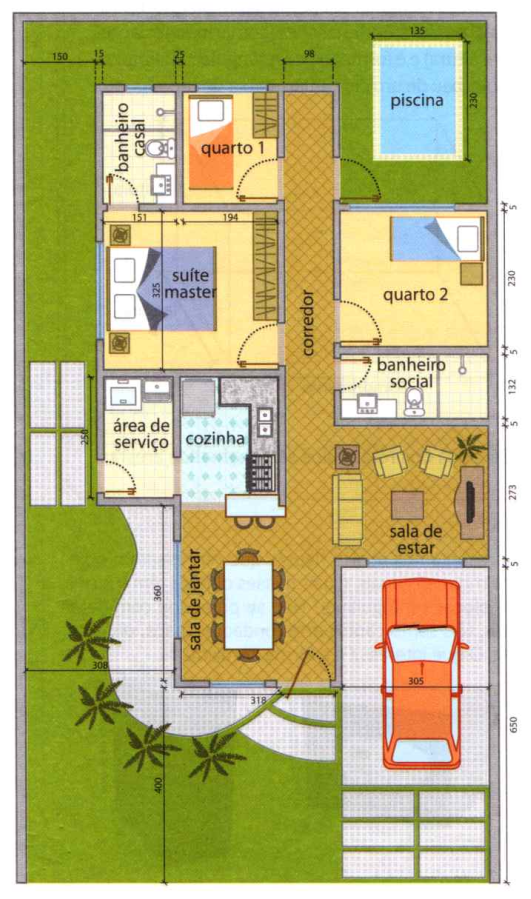
\includegraphics[width=1\linewidth]{6FMA30_imagens/imagem1}
		
	\end{multicols}
	\noindent\textsubscript{-----------------------------------------------------------------------------------------------------------------------------------------------------------}
	\begin{multicols}{2}
			\begin{enumerate} 
			\item Uma primeira informação importante que podemos obter da planta baixa é se a chamada área social da residência, ou seja, onde recebemos as visitas, é separada da área em que só costumam circular os moradores. Você diria que isso ocorre na planta baixa dada como exemplo na introdução da aula? \\ Justifique sua resposta. \\\\\\\\\\\\\\\\\\\\
			\item Quais cômodos têm portas para o exterior da residência? Como você explicaria a escolha desses locais para portas? \\\\\\\\\\\\\\\\\\\\
			\item As dimensões da planta baixa costumam estar em escala, ou seja, a relação entre as medidas na planta é a relação entre as medidas reais. Por exemplo, ao medirmos a dimensão horizontal dos dois quartos da residência representada abaixo, obteremos por volta de 2 cm. Podemos, então, afirmar que as dimensões horizontais reais dessas paredes são iguais. \\
			Em breve, aprenderemos o conceito de área, que nos permitirá responder às perguntas que formularemos a seguir com maior precisão: por enquanto, tentaremos respondê-las com os conceitos que já vimos.\\
			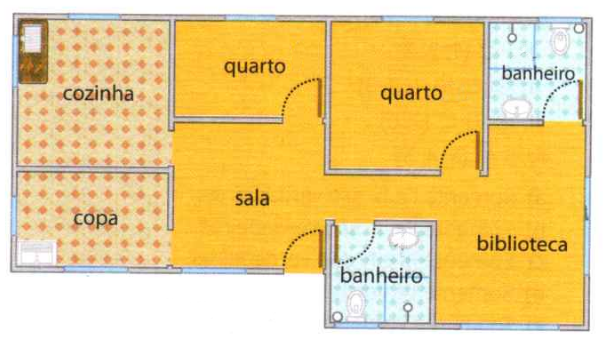
\includegraphics[width=1\linewidth]{6FMA30_imagens/imagem2} 
			\begin{enumerate}[a)]
				\item Desconsiderando a biblioteca, quais são os cômodos mais amplos (maiores) e os menos amplos (menores) da casa? \\\\\\\\\\\\\\\\\\\\
				\item Considere que na figura cada centímetro representa um metro na realidade. Qual é o comprimento do corredor que liga a sala à biblioteca? \newpage
			\end{enumerate}
			\item O que você observa de possivelmente errado na seguinte planta baixa? Há uma explicação para esse erro? \\
			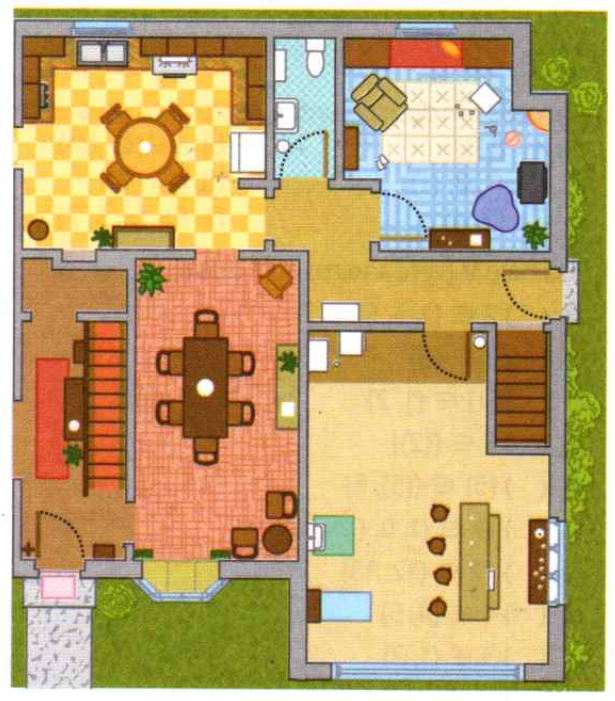
\includegraphics[width=1.1\linewidth]{6FMA30_imagens/imagem3} 
			\\\\\\\\\\\\\\\\\\\\\\\\\\\\\\\\\\\\\\\\\\\\\\
			\textbf{Desafio olímpico}
			\\
			\\
			(OBMEP) Vários quadrados foram dispostos uma ao lado do outro, em ordem crescente de tamanho, formando uma figura com 100 cm de base. O lado do maior quadrado mede 20 cm. Qual é o perímetro (medida do contorno em vermelho) da figura formada por esses quadrados? \\
			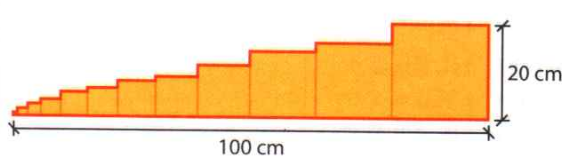
\includegraphics[width=1\linewidth]{6FMA30_imagens/imagem4} \\
			\begin{enumerate}[a)]
				\item 220 cm
				\item 240 cm
				\item 260 cm
				\item 300 cm
				\item 400 cm
			\end{enumerate}
			\newpage
			%107 a 110
			\item Considere a seguinte planta baixa, em que cada centímetro representa um metro. \\
			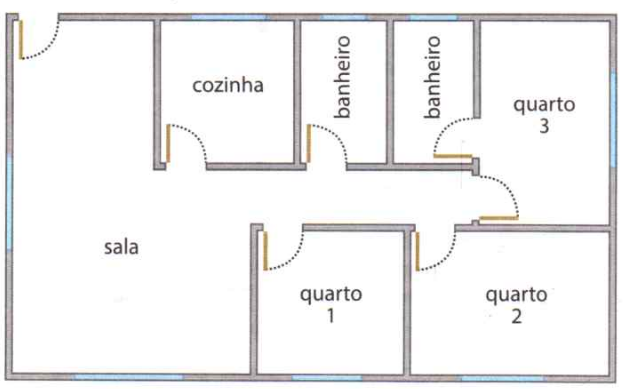
\includegraphics[width=1.1\linewidth]{6FMA30_imagens/imagem5}
			\begin{enumerate}[a)]
				\item Desconsiderando a sala, quais são os cômodos mais amplos? \\\\\\\\\\\\
				\item Qual é o quarto com menor perímetro? \\\\\\\\\\\\
			\end{enumerate}
			\item Pedro e seu irmão Júlio dividiam o quarto. Com a saída de Júlio de casa, seu irmão resolveu comprar uma estante para guardar sua coleção de livros e decidiu colocá-la na parede oposta à janela, onde ficava a cama de Júlio. A figura abaixo representa a planta baixa da casa dos irmãos antes da mudança de Júlio.\\
			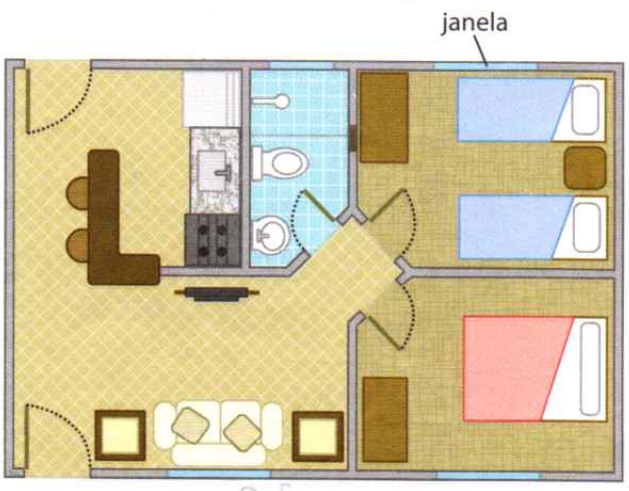
\includegraphics[width=1.1\linewidth]{6FMA30_imagens/imagem6} \\
			Considerando que cada centímetro equivale a dois metros na realidade, qual é o comprimento máximo que a estante deverá ter para ficar nessa parede?  \\\\\\\\\\\\
			\item O rodapé é uma pequena barra que se coloca ao longo das paredes na junção com o piso para fins decorativos. Ele pode ser feiro de vários materiais, sendo madeira o mais utilizado.  \\
			Ao comprar um novo apartamento, Ana optou por colocar rodapés nos quartos. A seguinte figura representa a planta baixa do seu novo apartamento, e as medidas dos quartos estão indicadas:\\
			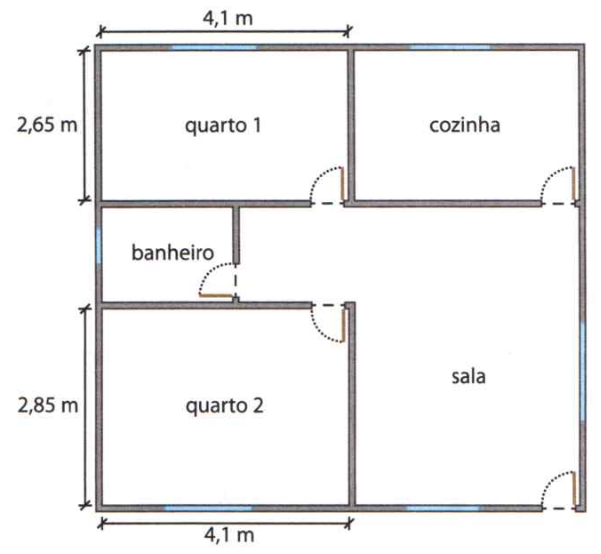
\includegraphics[width=1.1\linewidth]{6FMA30_imagens/imagem7}
			O rodapé escolhido por Ana custa R\$ 20,00 o metro e será aplicado em todas as paredes dos quartos, exceto na região das portas, que tem 70 cm de comprimento cada uma. Qual será o valor gasto por Ana?  \\\\\\\\\\\\\\\\\\\\\\\\\\\\\\\\\\\\\\\\\\\\
			\item Observe a seguinte planta baixa. \\
			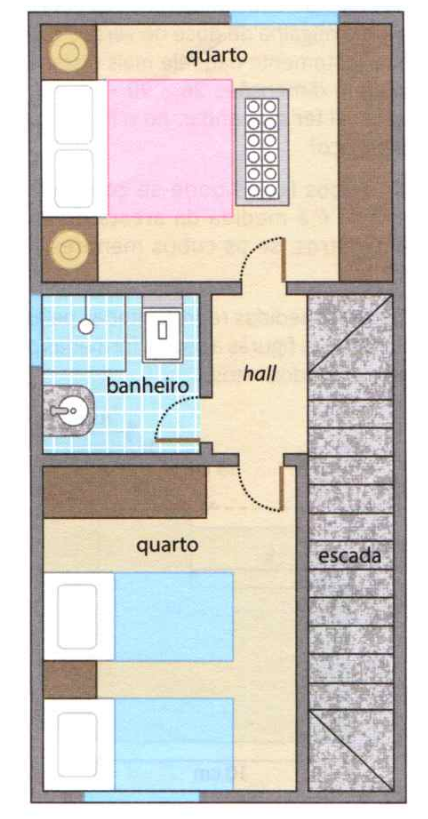
\includegraphics[width=1.1\linewidth]{6FMA30_imagens/imagem8}
			Quais cômodos não estão presentes nessa planta e qual seria uma explicação possível para isso?
			
			
		\end{enumerate}
		$~$ \\ $~$ \\ $~$ \\ $~$ \\ $~$ \\ $~$ \\ $~$ \\ $~$ \\ $~$ \\ $~$ \\ $~$ \\
	\end{multicols}
\end{document}